\begin{chapter}{\label{cha:shin}Decay of 2D quantum turbulence in a highly oblate Bose-Einstein condensate}
%%%%%%%%%%%%%%%%%%%%%%%%%%%%%%%%%%%%%%%%%%%%%
\newcommand{\gws}[1]{\textcolor{blue}{#1}}
\newcommand{\ngp}[1]{#1}%\textcolor{red}{#1}}
\newcommand{\etal}{{\it et al.}~}
\newcommand{\etalcc}{{\it et al.}}
\newcommand{\boldell}{{\mbox{\boldmath $\ell$}}}
\newcommand{\intr}{\int d \mathbf{r}}
\newcommand{\bfrt}{({\bf{r}},t)}
\newcommand{\fprt}{f({\mathbf{p}}, {\mathbf{r}},t)}

\section{Introduction}
Ultracold gaseous Bose-Einstein condensates (BECs) provide a unique testbed with which to investigate the phenomenon of quantum turbulence and the more rudimentary realm of superfluid vortex dynamics \citep{white_anderson_14,barenghi_skrbek_14}.  These systems provide an impressive degree of parameter manipulation unavailable in superfluid helium, the traditional context for studying quantum turbulence \citep{barenghi_donnelly_01}, with scope to control the particle interactions and potential landscape in both time and space.  The typical size of these systems is only one or two orders of magnitude larger than the inter-vortex spacing, which in turn is another order of magnitude larger than the vortex core size.  These compact length scales mean that the collective behaviour of vortices and their interaction with the background condensate is significant.  The emergence of turbulent-like behaviour in the form of a vortex tangle was observed by Henn {\it et al.} in 2009 by oscillating a three-dimensional condensate \cite{Henn}.  What's more, the experimentalist's handle over the confining potential enables crossover to two-dimensional quantum turbulence~\cite{parker2005}: by tightly confining the trap geometry along one axis, such that the vortices closely embody point vortices \cite{middelkamp}, states of two-dimensional quantum turbulence have been recently reported~\citep{neely_bradley_13,kwon_moon_14}.

In the recent experiment of Kwon {\it et al.} \citep{kwon_moon_14}, a trapped, oblate BEC was translated past a stationary, laser-induced obstacle.  As investigated in Chapter \ref{cha:wake}, vortices and anti-vortices were nucleated into the condensate once the relative speed exceeded a critical value~\cite{frisch92}, characteristic of superfluids. A state of two-dimensional quantum turbulence emerged, characterized by a disordered distribution of vortices.  The authors monitored the number of vortices, revealing the dependence on the relative speed and the thermal relaxation of the vortices.  They directly observed vortex collision events, characterized by a crescent-shaped depletion in the condensate density. Furthermore, some vortex cores were seen to coalesce, evidence of vortex pair annihilation.

 In this chapter we elucidate these experimental
findings through mean-field simulations of the two--dimensional Gross-Pitaevskii equation (GPE), both at zero-temperature and in the presence of 
thermal dissipation, modelled through a phenomenological dissipation term.  Notably, our simulations provide insight into the sign of the circulation of the vortices and the early-stage evolution, not accessible experimentally.  We establish the key stages of the dynamics, from the initial nucleation of vortices and formation of a quasi-classical wake, through the rapid symmetry breaking and disorganization of the vortices, to the decay of the vortices by annihilation or passage out of the condensate.  

\section{Model}
In the experiment, a $^{23}$Na condensate with $N=1.8\times 10^6$ atoms was confined within a highly-oblate cylindrically symmetric harmonic trap $V_{\mathrm{trap}}(x,y,z)=\frac{1}{2}m[\omega_r^2 (x^2+y^2) +\omega_z^2 z^2 ]$, with axial frequency $\omega_z=2 \pi \times 350$ Hz and radial frequency $\omega_r=2\pi \times 15$ Hz (corresponding to an aspect ratio parameter $\omega_z/\omega_r \approx 23$) and where $m$ denotes the atomic mass.  
A 2D mean-field description is strictly valid when 
the condition $N a l_z^3/l_r^3 \ll 1$ is satisfied, 
where $l_z=\sqrt{\hbar/m \omega_z}$ and $l_r=\sqrt{\hbar/m\omega_r}$ 
are the axial and radial harmonic oscillator lengths and $a$ is 
the {\it s}-wave scattering length \cite{delgado,parker2008}.  
For this experiment, $N a l_z^3/l_r^3=8.3$, i.e. the system remains 
3D in nature.   Nonetheless, the dynamics of the vortices is essentially 2D 
due to the suppression of Kelvin waves in 
the $z$-direction~\citep{jackson_proukakis_09}.  
Therefore, we will adopt a 2D description throughout this chapter and 
show that it is sufficient to capture the experimental observations.  
It is worth noting that in the $xy$ plane the condensate 
closely approximates a Thomas-Fermi (inverted parabola) density 
profile with radius $R_{\rm TF}\approx70 \mu m$.

We parametrise the condensate by the 2D wavefunction $\psi({\bf r},t)$; the condensate density distribution follows as $n({\bf r},t)=|\psi({\bf r},t)|^2$.  The wavefunction satisfies the GPE, Equation (\ref{eq:gpe}), as described in Section \ref{section:gpe}. For computational efficiency, the numerical simulations are performed using dimensionless quantities as described in Section \ref{section:gpedimlesstrap}. Quantities are made dimensionless by writing them in terms of the harmonic oscillator units: length in terms of the radial harmonic oscillator length $l_r$, energy in terms of $\hbar\omega_r$, and time in terms of inverse radial trapping frequency $\omega_r^{-1}$. However, to remain relevant to the experimental work of Shin \etal, in this chapter we report all quantities in their full dimensional form.

We solve the GPE on a $1024 \times 1024$ grid, with grid spacing $0.27\mu$m in both $x$ and $y$, using the fourth-order Runge-Kutta method described in Section \ref{section:RK4}. We have verified that reducing the grid spacing has no effect on our results. The vortex core size is characterized by the healing length $\xi=\hbar/\sqrt{m n g}$; at the condensate centre this has the value $\xi \approx 0.6 \mu$m.

Following the experiment, the total potential acting on the condensate, $V({\bf r},t)$, is the above harmonic trap plus a static Gaussian-shaped circular obstacle potential of the form described in Section \ref{section:3dcylinderpotential},
\begin{equation}
  V_{\rm{obj}}({\bf r}) = V_0 \exp\left ( -\frac{(x-x_0)^2}{d^2}-\frac{y^2}{d^2}\right ),
\end{equation}
with $V_0=15 \mu$ and $d=11.31\mu$m.  The initial ground-state BEC is obtained by solving the GPE using the imaginary time method shown in Section \ref{section:imagTime}, with an enforced norm of $N=1.8\times 10^6$ to match the experimental value.  At $t=0$ the harmonic trap is centred at $x_0=18.5\mu$m. The trap is translated towards the left, at speed $v$, over a distance of $37 \mu$m; to smooth this speed curve we additionally include a linear acceleration/deceleration over $3.75$ms at the start/end, which is included as part of the $37\mu$m translation.  Once the trap is at rest, the obstacle amplitude $V_0$ is ramped down to zero over $0.4$s.

\section{Number of Vortices Generated}
\begin{figure}
\begin{center}
  \begin{tikzpicture}
  \begin{axis}[ylabel near ticks,xlabel near ticks,
        width=0.5\linewidth,
        xtick pos=left,
      ytick pos=left,
        xlabel=$v$ (mm/s),
        ylabel=$N_v$,
        xmin=0.2,
        xmax=1.8,
        ymin=0,
        ymax=100,
        major tick length = 0.07cm,
        samples=300
      ]
      %\addplot+[only marks, error bars/y dir=both, error bars/y fixed=3,error bars/error bar style={thick}] file {shin/nv_v_lowtemp.dat};
      %\addplot+[only marks, error bars/y dir=both, error bars/y fixed=3,error bars/error bar style={thick},color=red,mark=square*,every mark/.append style={solid, fill=red}] file {shin/nv_v_hightemp.dat};
      \addplot+[only marks] file {shin/nv_v_lowtemp.dat};
      \addplot+[only marks,color=red,mark=square*,every mark/.append style={solid, fill=red}] file {shin/nv_v_hightemp.dat};
      \addplot+[only marks,color=black,mark size = 2, mark=diamond*,every mark/.append style={solid, fill=black}] file {shin/nv_v_exp.dat};
      \addplot+[mark=none,color=red,solid] {(85.2084 / (1 + exp(-8.4940*x + 5.6354))-4.6183)};
      \addplot+[mark=none,color=blue,solid] {(61.2430 / (1 + exp(-14.7576*x + 10.4699))-0.7081)};
      \addplot+[mark=none,color=black,solid] {(64.6833 / (1 + exp(-7.8208*x + 5.5874))-2.1150)};
    \end{axis}
\end{tikzpicture}
\end{center}
\caption{\label{fig:N_vV} Number of vortices $N_v$ in the condensate after removal of the obstacle. Shown are simulations of the GPE without dissipation (red squares), with dissipation $\gamma = 0.0003$ (blue circles) and experimental results extracted from Figure 1 of~\citep{kwon_moon_14} (black diamonds). Sigmoid fits are also shown as dashed lines. Each point is averaged over $20$ ms once the obstacle amplitude reaches $V_0=0$.  For comparison, the speed of sound in the centre of the BEC is $v_c\approx 4.6$ mm/s.  }
\end{figure} 
Following removal of the obstacle, we determine the number of vortices in the system $N_v$ using the methods described in Section \ref{section:vortexidentifying}.  
We limit our search to $75$ percent of the Thomas-Fermi radius \ngp{(centred on the centre-of-mass to account for sloshing motion)}; by avoiding the low density periphery we avoid artefacts from ghost vortices and match closely what is performed experimentally (since vortices close to the edge are not detected due to low signal-to-noise~\citep{shin_private}). 

In Figure \ref{fig:N_vV} we plot $N_v$ versus the translation speed $v$.  We see the same {\it qualitative} form between our simulations (red squares) and the experiment (black diamonds): above a critical speed $v_c \approx 0.45$mm/s vortices enter the system, nucleated by the relative motion between the obstacle and the superfluid, and for $v>v_c$ the growth in $N_v$ is initially rapid but tails off for $v\gg v_c$. Quantitatively, however, the GPE overestimates $N_v$.   One can expect that thermal dissipation, not accounted for in the GPE, will act to reduce the number of vortices in the system. Experimental limitations in resolving and counting vortices may also contribute to the over-estimate of $N_v$ from the GPE.

We include the effects of dissipation via the addition of phenomenological dissipation~\citep{choi_morgan_98,tsubota_kasamatsu_02}, $\gamma$, which enters the GPE by replacing $i$ on the left hand side by $(i-\gamma)$, a process formally derived in Section \ref{section:dgpe}.  This term induces the decay of excitations; for single vortices this manifests in them spiralling out of the trapped condensate~\citep{madarassy_barenghi_08,jackson_proukakis_09,allen_zaremba_13,yan_proukakis_14}. We choose a small value $\gamma = 0.0003$ so as to model the experiment in its very coldest realization of $T\sim130$nK and enforce the norm throughout the dissipative simulations so as to emulate the experiment (for which no significant loss of atom number was observed). With this dissipation the data for $N_v$ becomes reduced (blue circles), bringing it closely in line with the experimental data.

\section{Stages of the Condensate Evolution}

We now examine in detail the evolution of the condensate, 
charting its dynamics from the initial stage (when the
harmonic trap translation begins) to the intermediate and final stages 
(randomization and decay of the vortices).  We see the same 
qualitative evolution with and without dissipation, and for all 
velocities exceeding $v_c$.  For the purposes of illustration, 
we focus on an example with dissipation and a translation 
speed $v=1.4$mm/s. 

\begin{figure}
\centering
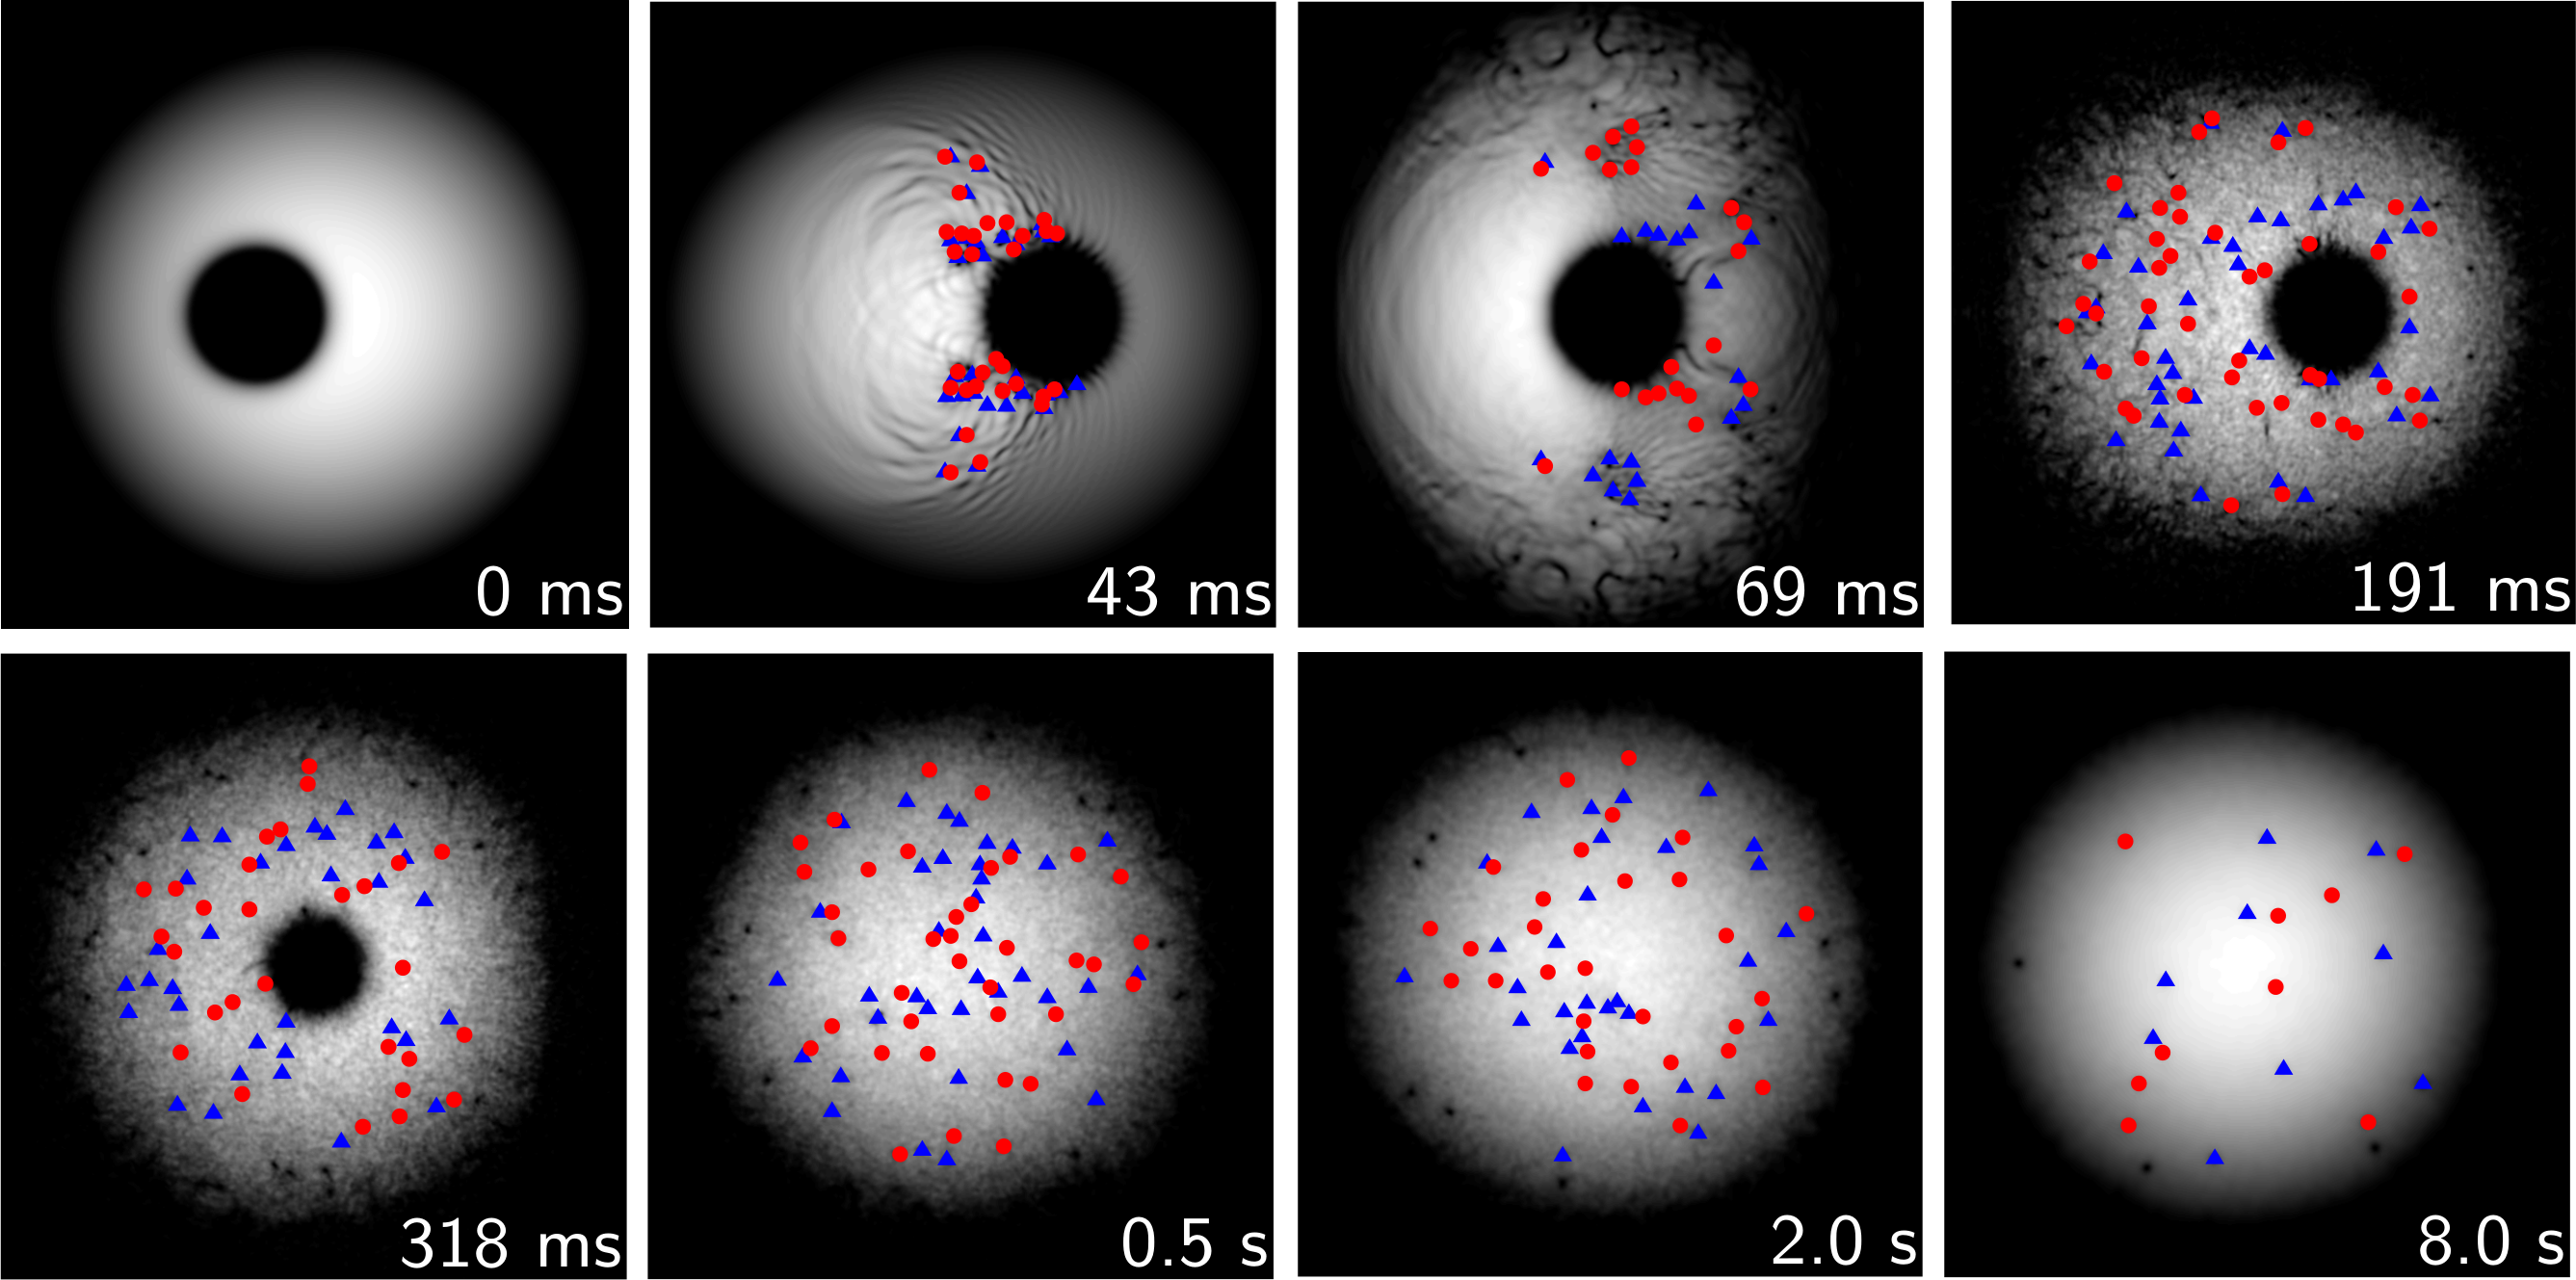
\includegraphics[width=0.95\linewidth]{shin/fig2_4x2}
\caption{\label{fig:densSnapshots} Snapshots of the condensate density, for a translational speed $v=1.4$mm/s and in the presence of dissipation ($\gamma=0.0003$). The obstacle is completely removed at $0.43$s. The field of view in each subfigure is of size $[170\mu$m$]^2$ and shifted along the $x$-axis so as to best display the condensate.  Vortices with positive (negative) circulation are highlighted by red circles (blue triangles).
}
\end{figure}

Figure \ref{fig:densSnapshots} shows the condensate density at various times. At the start of the simulation ($t=0$) the condensate has a smooth circular density profile, with a density depression due to the obstacle.  Later vortices appear as small dots of low density; superimposed red/blue markers identify vortices of positive/negative circulation.

\subsection{Vortex Nucleation and Wake Formation}

To initiate the dynamics, the harmonic trap is translated to the left.  This is performed sufficiently rapidly that the condensate does not adiabatically follow the trap minimum, but rather begins a sloshing motion in the trap; the centre-of-mass of the BEC oscillates at the trap frequency and the BEC undergoes a quadrupolar shape oscillation. As the BEC sloshes first to the left, its speed increases.  When the local fluid velocity exceeds the speed of sound, vortices nucleate \cite{frisch92} at the poles of the obstacle
(where the local fluid velocity is the greatest) 
and are washed downstream (to the left).  
As seen in Chapter \ref{cha:wake}, the pattern of vortices nucleated by a moving obstacle 
in a superfluid depends, in general, on the  speed, shape and size of 
the obstacle~\citep{jma00,saito10,stagg_parker_14}. 
During the initial evolution vortices of negative
and positive circulation are created near each pole in an 
irregular manner, sometimes with alternating circulation;  
other times several vortices of the same circulation appear.
During this early stage ($t=43$ms), vortices of opposite 
circulation may become very close and annihilate (i.e. undergo 
a 2D reconnection), leaving behind density (sound) waves.
The condensate then sloshes to the right; this 
motion not only carries the existing vortices to the opposite 
(right) side of the obstacle but nucleates further vortices.
%In our case, the rate of vortex nucleation is sufficiently 
%high that the vortices interact strongly with each other, 
%collectively forming macroscopic clusters of negative and positive 
%vortices near the object ($t=69$ms).  This is reminiscent of the wakes in classical viscous fluids past cylindrical obstacles \cite{stagg_parker_14}.  
As the condensate's sloshing mode is damped by 
the dissipation, the relative speed of the obstacle decreases
and the vortex nucleation pattern changes: 
like-signed vortices are generated near each pole. 
In our case, the rate of vortex nucleation is sufficiently 
high that the like-sign vortices interact strongly with each other, 
collectively forming macroscopic clusters of negative and positive 
vortices near the object ($t=69$ms).  This is reminiscent of the wakes in classical viscous fluids past cylindrical obstacles \cite{stagg_parker_14}. 
%This effect leads to further clustering of like-signed vortices   
%($t=69$ms).
As the condensate continues to slosh, more
vortices nucleate into the system. It must be stressed that,
up to these early times ($t=191$ms), the vortex distribution remains symmetric 
about the $x$ axis.

Without the dissipation term in the GPE, the sloshing mode initially decays while the obstacle is present but then persists with constant amplitude once the obstacle is removed.  If dissipation is included then the sloshing mode continues to decay. Figure \ref{fig:com_slosh} shows the centre-of-mass oscillation over time, demonstrating the decay and that in either case, the sloshing mode is produced at the trap frequency.
\begin{figure}
\begin{center}
  \begin{tikzpicture}
  \begin{axis}[ylabel near ticks,xlabel near ticks,
        width=0.5\linewidth,
        xtick pos=left,
        ytick pos=left,
        xlabel={Time (s)},
        ylabel={Centre-of-mass ($\mu$m)},
        xmin=0,
        xmax=1.9,
        major tick length = 0.07cm
      ]
      %\addplot+[mark=none,color=red] {(85.2084 / (1 + exp(-8.4940*x + 5.6354))-4.6183)};
      \addplot+[mark=none,color=blue,thick] file {shin/com_gpe.dat};
      \addplot+[mark=none,color=red,thick] file {shin/com_dgpe.dat};
    \end{axis}
\end{tikzpicture}
\end{center}
\caption{\label{fig:com_slosh} Centre-of-mass oscillations during condensate evolution for the BEC without the dissipation term (blue), and with a dissipation of $\gamma = 0.0003$ (red).}
\end{figure} 

\subsection{Vortex Randomization}
In the presence of the obstacle and the sloshing mode,
vortices continually nucleate and their spatial distribution remains
approximately symmetric about the $x$ axis.  
At later times ($t>318$ms) this symmetry breaks and the vortices 
evolve into a completely disorganised, apparently random 
configuration with no significant clustering of like-signed vortices.  \ngp{This random distribution of vortices is consistent with the experimental observations \cite{kwon_moon_14}; following this we also classify the system as one of quantum turbulence.
Besides vortices, the condensate contains also collective modes and
an energetic, disordered sound field, with this spatial range of excitations further indicative of two-dimensional 
quantum turbulence \cite{parker2005,neely_bradley_13}. (Note that the typical characteristic diagnostics of steady-state 2D quantum turbulence, e.g. power-law energy spectra and the inverse energy cascade, are not appropriate here since the system is not continuously driven and does not reach steady state.)}

\ngp{The vortex randomization is driven by the growth of numerical noise.  We have repeated our results in the presence of imposed noise (amplitude $5\%$, as described elsewhere \cite{stagg_parker_14}) and find the qualitative dynamics to be unchanged (although, as one would expect, the vortex randomization occurs at a slightly earlier time).  This noise serves to model the natural fluctuations that arises in a realistic experimental scenario, e.g. due to thermal and quantum atomic fluctuations, electromagnetic noise, vibrations, etc.}

It is interesting to note the obstacle is still in the system 
at this point, nucleating vortices in a symmetrical manner. 
The disorganised vortices already in the system create a velocity 
field which quickly mixes newly created vortices nucleated at the
poles of the obstacle. Visual inspection, confirmed by the RCA clustering-detection algorithm~\citep{white12,reeves_billam_13} described in Section \ref{section:reevesalgorithm}, 
shows no significant clusters beyond this stage of the evolution. 
By the time the obstacle is removed the vortex configuration is 
essentially random, but 
the number of positive and negative vortices stays approximately equal.
It is important to remark that, without detecting the sign of the vortex circulation, we
could not reach these conclusions.

\begin{figure}
\begin{center}
  \begin{tikzpicture}
  \begin{axis}[ylabel near ticks,xlabel near ticks,
        width=0.5\linewidth,
        xtick pos=left,
        ytick pos=left,
        xlabel={Time (s)},
        ylabel=$N_v$,
        xmin=0,
        xmax=0.5,
        ymin=0,
        ymax=90,
        major tick length = 0.07cm
      ]
      \addplot+[mark=none,color=blue,thick] file {shin/nv_t_lowtemp.dat};
      \addplot+[mark=none,color=red,thick] file {shin/nv_t_hightemp.dat};
    \end{axis}
\end{tikzpicture}
\end{center}
\caption{\label{fig:N_vTime} Growth of vortex number (in a single realization) at early times for a translational speed of $v=1.4$mm/s. Shown are the results with no dissipation (blue) and with dissipation $\gamma=0.0003$ (red).}
\end{figure}

\subsection{Vortex Decay}
It is clear from Figure \ref{fig:densSnapshots} that, following the removal 
of the obstacle, the number of vortices, $N_v$, depletes.   
Indeed, one expects that the condensate will decay towards its 
vortex--free, time--independent ground state.  To quantify the vortex generation and
decay, Figure \ref{fig:N_vTime} plots the growth of $N_v$ at early times, 
and Figure \ref{fig:N_vLong} (a, b) plots the decay of vortices over the remaining experimental time period. 
The onset of vortex nucleation is at around $t=0.02$ms; 
this is the time taken for accelerating condensate to exceed the speed of 
sound at the poles of the object.
At first $N_v$ grows steeply, as vortices (around 40-60) are rapidly driven into the system. Subsequently, $N_v$ grows more slowly; vortices continue to be nucleated from the obstacle but vortices undergo annihilation or move into low density regions where they are not detected.  The fluctuations in $N_v$ are amplified, particularly at early times, by the shape oscillations of the condensate, which carry vortices in and out of the detection radius. As the obstacle is removed, the surrounding condensate fills the low density area. Vortices (including some outside of the detection radius) move inwards with the condensate, causing $N_v$ to peak at $t\approx 0.4$s. Following removal of the obstacle, the vortex number $N_v$ decays with time.  This is shown in Figure \ref{fig:N_vLong}(a) and (b) for the absence and presence of dissipation, respectively.

\begin{figure}
\begin{center}
(a)\hspace{0.45\linewidth}(b)\hspace{0.4\linewidth}~\\
  \begin{tikzpicture}
  \begin{axis}[ylabel near ticks,xlabel near ticks,
        width=0.45\linewidth,
        xtick pos=left,
        ytick pos=left,
        xlabel={Time (s)},
        ylabel=$N_v$,
        xmin=0.45,
        xmax=8,
        ymin=0,
        ymax=82,
        xtick={0.5, 2, 4, 6 ,8},
        axis on top,
        major tick length = 0.07cm
      ]
      \addplot [thick,color=red,mark=none,draw=none,fill=red!60]coordinates {(100, 100) (100, 0) (0, 0) (0, 100)};
      \addplot[mark=none,draw=none,thick,fill=cyan!70] file {shin/nv_t_a_split.dat}\closedcycle;
      \addplot[mark=none,color=black,thick,fill=white] file {shin/nv_t_a_lower.dat}\closedcycle;
      \node[anchor=west] at (axis cs:  1.25,  77) {\sf Drift};
      \node[anchor=west] at (axis cs:  1.25,  55) {\sf Annihilation};
    \end{axis}
\end{tikzpicture}
\begin{tikzpicture}
  \begin{axis}[ylabel near ticks,xlabel near ticks,
        width=0.45\linewidth,
        xtick pos=left,
        ytick pos=left,
        xlabel={Time (s)},
        ylabel=$N_v$,
        xmin=0.45,
        xmax=8,
        ymin=0,
        ymax=64,
        xtick={0.5, 2, 4, 6 ,8},
        axis on top,
        major tick length = 0.07cm
      ]
      \addplot [thick,color=red,mark=none,draw=none,fill=red!60]coordinates {(100, 100) (100, 0) (0, 0) (0, 100)};
      \addplot[mark=none,draw=none,thick,fill=cyan!70] file {shin/nv_t_b_split.dat}\closedcycle;
      \addplot[mark=none,color=black,thick,fill=white] file {shin/nv_t_b_lower.dat}\closedcycle;
      \node[anchor=west] at (axis cs:  2,  58) {\sf Drift};
      \node[anchor=west] at (axis cs:  2,  40) {\sf Annihilation};
    \end{axis}
\end{tikzpicture}\\%
(c)\hspace{0.45\linewidth}(d)\hspace{0.4\linewidth}~\\
\begin{tikzpicture}
  \begin{axis}[ylabel near ticks,xlabel near ticks,
        width=0.45\linewidth,
        xtick pos=left,
        ytick pos=left,
        xlabel={Time (s)},
        ylabel={\# Vortices Removed},
        xmin=0.45,
        xmax=8,
        ymin=0,
        ymax=61,
        xtick={0.5, 2, 4, 6 ,8},
        axis on top,
        major tick length = 0.07cm
      ]
      \addplot[mark=none,color=red] file {shin/nv_t_c_drift.dat};
      \addplot[mark=none,color=blue] file {shin/nv_t_c_an.dat};
      \addplot[mark=none,color=red,ultra thick,dashed] file {shin/nv_t_c_drift_fit.dat};
      \addplot[mark=none,color=blue,ultra thick,dashed] file {shin/nv_t_c_an_fit.dat};
    \end{axis}
\end{tikzpicture}%
\begin{tikzpicture}
  \begin{axis}[ylabel near ticks,xlabel near ticks,
        width=0.45\linewidth,
        xtick pos=left,
        ytick pos=left,
        xlabel={Time (s)},
        ylabel={\# Vortices Removed},
        xmin=0.45,
        xmax=8,
        ymin=0,
        ymax=32,
        xtick={0.5, 2, 4, 6 ,8},
        axis on top,
        major tick length = 0.07cm
      ]
      \addplot[mark=none,color=red] file {shin/nv_t_d_drift.dat};
      \addplot[mark=none,color=blue] file {shin/nv_t_d_an.dat};
      \addplot[mark=none,color=red,ultra thick,dashed] file {shin/nv_t_d_drift_fit.dat};
      \addplot[mark=none,color=blue,ultra thick,dashed] file {shin/nv_t_d_an_fit.dat};
    \end{axis}
\end{tikzpicture}%
\end{center}
\caption{\label{fig:N_vLong} Vortex decay in the absence of dissipation (a, c) and with dissipation $\gamma=0.0003$ (b, d) for a translational speed of $v=1.4$mm/s.  The upper figures show the decay of the total vortex number $N_v(t)$, with the contribution of drifting and annihilation depicted by the shaded regions.  The lower figures show the drift number $N_d(t)$ and annihilation number $N_a(t)$, plus their respective fits.}
\end{figure}

\subsubsection{Kwon's decay model}\label{kwon_fitting}
Kwon {\etal}\citep{kwon_moon_14} argued that there are two mechanisms 
by which vortices decay: (i) thermal dissipation
(resulting in drifting of vortices to the edge of the condensate),
and (ii) vortex-antivortex annihilation events, and proposed
that the vortex decay takes the form:
\begin{equation}
\frac{{\rm d}N_v}{{\rm d}t}= - \Gamma_1 N_v - \Gamma_2 N_v^{~2}.
\label{eqn:N_v_decay}
\end{equation}
Here the linear and nonlinear terms, parametrised by the positive
coefficients $\Gamma_1$ and $\Gamma_2$, respectively, model
these two decay processes.  From our simulations we are able to independently count the number of vortices which drift out and the number which annihilate.  
We decompose the number of vortices according to 
\begin{equation}
  N_v(t) = N_i - N_d(t) - N_a(t),
\label{eqn:N_v_decomp}
\end{equation}
where $N_i$ is the initial number of vortices (when the obstacle is removed), $N_d(t)$ is the cumulative number of vortices which have drifted out of the condensate and $N_a(t)$ is the cumulative number which have undergone pair annihilation.
The contribution of both vortex drifting and annihilation to the overall decay of $N_v$ is depicted by the coloured regions in Figure \ref{fig:N_vLong}(a) and (b).  In the absence of dissipation  the vortex decay is dominated by annihilation.  Indeed, apart from at early times (where internal condensate dynamics carry vortices out to high radii), no vortices drift out.  In contrast, in the presence of dissipation, vortices continue to drift out over time, consistent with dissipative dynamics of single vortices \citep{allen_zaremba_13}.

Unfortunately, fitting $N_v(t)$ directly to Equation (\ref{eqn:N_v_decay}) leads to inconclusive results. While we find that the best-fitting solutions fit the data well, the resulting values for $\Gamma_1$ are found to be negative, corresponding to a positive growth. Considering that $\Gamma_1$ is a term associated to thermal dissipation there is no reason to expect a growth here. We interpret this inconsistency as resulting from fitting Equation (\ref{eqn:N_v_decay}) directly; the meaning of the rates $\Gamma_1$ and $\Gamma_2$ (i.e as characterising rates of vortex loss through drifting and vortex-antivortex annihilation) are not enforced, and so the best-fit parameters cannot be used to infer anything about the physical processes.

Our solution is to enforce the meaning of $\Gamma_1$ and $\Gamma_2$ while performing the fitting process. The decomposition of $N_v$ as Equation (\ref{eqn:N_v_decomp}) enables us to independently fit the drift and annihilation decay processes as two coupled ODEs for $N_d$ and $N_a$,
\begin{equation}
  \frac{{\rm d}N_d}{{\rm d}t} = \Gamma_1 N_v,~~~~~~~~~~~~~~
  \frac{{\rm d}N_a}{{\rm d}t} = \Gamma_2 N_v^{~2}.
\label{eqn:N_v_couple}
\end{equation}
By taking the time derivative of Equation (\ref{eqn:N_v_decomp}) and substituting in Equation (\ref{eqn:N_v_couple}), Equation (\ref{eqn:N_v_decay}) can be recovered. As a consequence of fitting the coupled ODEs independently, the physical meaning of each rate term is enforced. To further fix the physical meaning, the fitted value of both $\Gamma_1$ and $\Gamma_2$ are forced to be positive (corresponding to a vortex decay over time). The vortex decomposition along with the each independent fit is shown in Figure \ref{fig:N_vLong}(c) and (d) for the absence and presence of dissipation, respectively. We find that the rate equation fits fairly well most cases, although finds difficulty in fitting the lack of vortex decay via drifting when $\gamma=0$.

In the absence of dissipation we find a value of $\Gamma_{1} = 5.5 \times 10^{-2}$. However, it is not appropriate to discuss the physical meaning of $\Gamma_1$ in this case, since $\gamma=0$ and so $N_d$ is not of a decaying form; this also explains the less successful fit for $N_d$ in the absence of dissipation. We also find the corresponding $\Gamma_{2} = 9.7 \times 10^{-3}$. While the experimental observations \cite{kwon_moon_14} suggest $\Gamma_2$ is proportional to $T^2$ and thus approaches 0 as $T\rightarrow0$, our results demonstrate a finite $\Gamma_2$ in this limit.

With the inclusion of a dissipation of $\gamma=0.0003$ we obtain $\Gamma_{1} = 12.3 \times 10^{-2}$, this corresponds to an increase to the rate of vortex decay via the drifting out mechanism, as expected when introducing dissipation into the system \citep{allen_zaremba_13}. We also find $\Gamma_{2} = 5.3 \times 10^{-3}$. These values are in good agreement with the values obtained by Kwon \etal when fitting to their coldest experiments. 

\subsubsection{Modified decay model}
We have shown that the rate equation proposed by Kwon \etal \citep{kwon_moon_14}, Equation (\ref{eqn:N_v_decay}), can be used to characterise the decay of vortices via two mechanisms: a rate of decay due to drifting, and a rate of decay due to annihilation. However, to obtain physically realistic fits, we were forced to enforce the meaning of the two decay terms as part of the fitting mechanism, a process which is not ideal.%It is perhaps to be expected that such a simple rate equation would not capture the full spectrum of rich behaviour available to the GPE. It would be beneficial, however, to attempt to deeper understand the vortex-antivortex annihilation process and produce a higher quality universal decay law.

Post publication \cite{stagg_allen_14} of the results in this chapter, several authors \cite{Cidrim15,Groszek15} independently investigated vortex interactions in the context of quantum turbulence, providing arguments and evidence to support modified rate equations for the decay of vortex number in atomic BEC experiments. Recently, Cidrim \etal \cite{Cidrim15} proposed a scheme for generating two-dimensional quantum turbulence with the novelty of controlling the {\it polarisation} of the resulting turbulence by the addition of small localised repulsive potentials. Similarly to our findings in Section \ref{kwon_fitting}, fitting to Equation (\ref{eqn:N_v_decay}) without enforcing the meaning of the terms provided physically unrealistic decay rates. Cidrim \etal proposed a simple argument that takes into account the polarised nature of the turbulence and early-time steeper-than-quadratic effects, providing the following phenomenological model of vortex decay,
\begin{align}
\begin{split}
  \frac{{\rm d}N_+}{{\rm d}t} &= -\Gamma_3 N_+^{~3/2} -\Gamma_4(N_+N_-)^{2},\\
  \frac{{\rm d}N_-}{{\rm d}t} &= -\Gamma_3 N_-^{~3/2} -\Gamma_4(N_+N_-)^{2},
\end{split}
\label{eq:dnpdt_dnmdt}
\end{align}
where $N_+$/$N_-$ are the number of vortices of positive/negative circulation, so that $N_v = N_+ + N_-$. Fitting to this model gave physically realistic values for both decay rates in all of their simulated cases. For the unpolarised turbulence that we investigate, Equation (\ref{eq:dnpdt_dnmdt}) can be equivalently written as
\begin{equation}
  \frac{{\rm d}N_v}{{\rm d}t} = -\Gamma_3 N_v^{~3/2} -\frac{\Gamma_4}{8}N_v^{~4}.
  \label{eqn:N_v_cidrim}
\end{equation}
Groszek \etal independently provided evidence \cite{Groszek15} that vortex annihilation events are in fact a four-body loss mechanism, leading to an annihilation decay rate of the form ${{\rm d}N_v}/{{\rm d}t}\sim -N_v^4$, supporting the findings of Cidrim \etal

\begin{figure}
\begin{center}
  \begin{tikzpicture}
  \begin{axis}[ylabel near ticks,xlabel near ticks,
        width=0.45\linewidth,
        xtick pos=left,
        ytick pos=left,
        xlabel={Time (s)},
        ylabel=$N_v$,
        xmin=0.45,
        xmax=8,
        ymin=0,
        ymax=64,
        axis on top,
        major tick length = 0.07cm
      ]
      \addplot[mark=none,color=black,thick] file {shin/nv_t_b_lower.dat};
      \addplot[mark=none,color=blue,dashed,ultra thick] file {shin/nv_t_b_kwonfit.dat};
      \addplot[mark=none,color=red,dashed,ultra thick] file {shin/nv_t_b_kwonforcefit.dat};
      \addplot[mark=none,color=green,dashed,ultra thick] file {shin/nv_t_b_cidrimfit.dat};
    \end{axis}
\end{tikzpicture}
\end{center}
\caption{\label{fig:fitting_comp} Comparison of the three vortex decay models introduced in this chapter. Shown is the decay of vortex number for out GPE simulation with dissipation $\gamma=0.0003$ and a translational speed of $v=1.4$mm/s. (black solid line). Also shown is fits to the data using Kwon's rate equation (blue dashed line), Kwon's rate equation while enforcing the meaning of the decay rates (red dashed line) and Cidrim's equation (green dashed line).}
\end{figure}

As a further test of Cidrim's modified decay law we have fitted $\Gamma_3$ and $\Gamma_4$ to our simulation with dissipation $\gamma=0.0003$ and trap speed $v=1.4$mm/s. A comparison of the resulting decay rates is shown in Table \ref{tbl:fitting_comp}, and the fits are visually compared in Figure \ref{fig:fitting_comp}. Kwon's equation [Equation (\ref{eqn:N_v_decay})] provides a good qualitative fit to the decay rate overall, but physical processes cannot be inferred from the resulting values of the decay rates $\Gamma_1$ and $\Gamma_2$. Enforcing the meaning of the terms in Kwon's equation by fitting $N_d(t)$ and $N_a(t)$ independently [Equation (\ref{eqn:N_v_couple})] performs the least favourably overall, but provides physically realistic decay rates. Finally, Cidrim's equation [Equation (\ref{eqn:N_v_cidrim})] qualitatively fits {\it at least} as well as Kwon's equation, while having the advantage of physically realistic values for the decay rates and the ability to handle non-zero turbulence polarity. We note that our resulting values for $\Gamma_3$ and $\Gamma_4$ when fitted to Cidrim's equation compare well to values obtained by Cidrim \etal when fitting to decaying 2D turbulence with zero polarisation and $N_v(0) \sim 150$. These results suggest that of the fitting methods described, Cidrim's Equation is the best performing phenomenological model of vortex decay.

\begin{table}
\centering
\begin{tabular}{r|ccc}
{\it Decay rate} & {\it Kwon's equation} & {\it Decomposed Kwon's equation} & {\it Cidrim's equation} \\
\hline 
\rule{0pt}{3ex} Drift        & $\Gamma_1 = -1.8\times 10^{-1}$ & $\Gamma_1 = 12.3 \times 10^{-2}$ & $\Gamma_3 = 2.0 \times 10^{-2}$ \\
\rule{0pt}{3ex} Annihilation & $\Gamma_2 = 1.4\times 10^{-2}$ &  $\Gamma_2 = 5.3 \times 10^{-3}$  & $\Gamma_4 = 3.3 \times 10^{-6}$ \\
\end{tabular}
\caption{\label{tbl:fitting_comp} Comparison of the resulting decay rates when fitting Kwon's equation [Equation (\ref{eqn:N_v_decay})], decomposed Kwon's equation [Equation (\ref{eqn:N_v_couple})] and Cidrim's equation [Equation (\ref{eqn:N_v_cidrim})] to the decay of vortex number for our GPE simulation with dissipation $\gamma=0.0003$ and a translational speed of $v=1.4$mm/s.}
\end{table}

\section{Crescent-Shaped Density Structures}
In the experiment, Kwon \etal observed the occasional appearance of crescent-shaped waves of 
depleted density.  Lacking direct access to the vortex signs,
they suggested that these structures result from
annihilation events of vortices of opposite 
circulation~\citep{nazarenko_onorato_07,rorai_skreenivasan_12,prabhakar_singh_13}: a vortex reconnection is predicted to 
induce an intense, localised, rarefaction 
sound pulse~\cite{leadbeater,zuccher}.  
Figure~\ref{fig:cresentPlots} shows snapshots of the condensate density 
and phase during a reconnection event. Vortices show up as localized dips 
in the density (upper row) and $2 \pi$-defects in the phase (lower row). 
Figure~\ref{fig:cresentPlots} (a) shows a vortex (A) and antivortex (B) 
close to each other, and a third vortex (C) in the vicinity.
Note that the individual vortices are not spatially resolvable 
through their density alone (the vortex cores merge into a deep, elongated 
crescent-shaped depression), but they are clearly identified by the 
phase plot.  A short time later (b), vortices A and B annihilate, 
as confirmed by the disappearance of their phase singularities, 
leaving behind a shallow rarefaction pulse (S) with a linear phase step.  
This pulse rapidly evolves into a shallow, 
crescent-shaped sound wave [Figure \ref{fig:cresentPlots} (c)].  
\ngp{In other words, our simulations yield crescent-shaped density features 
as seen in the experiment, but these features are not uniquely formed 
by annihilation events - they may also result from from two (or more) 
vortices in close proximity.  Information about the condensate phase 
is thus crucial to distinguish the nature
of these observed structures.  In this direction, an approach has recently been proposed for the experimental detection of quantized vortices and their circulation in a 2D BEC \cite{powis}.}

%\begin{figure}
%\centering
%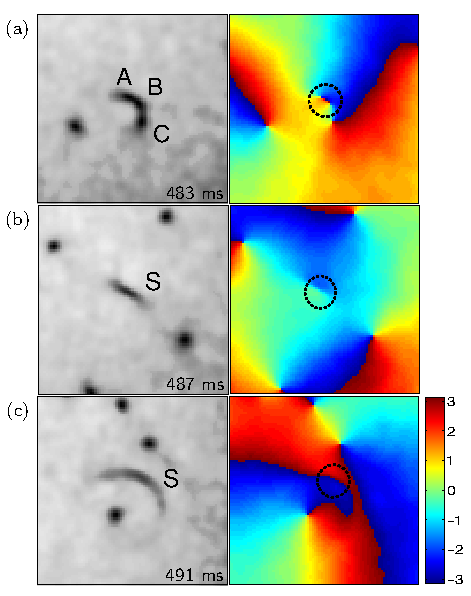
\includegraphics[width=0.9\linewidth]{shin/fig5}
%\caption{\label{fig:cresentPlots} Density (left) and phase (right) just before (a), immediately following (b) and a later time after (c) a vortex-antivortex annihilation event.  The field of view is  $[23.5\mu$m]$^2$, centered on the vortex pair/sound pulse (highlighted by a circle in the phase).}
%\end{figure}
\begin{figure}
\hspace*{0.07\linewidth}(a)\hspace{0.23\linewidth}(b)\hspace{0.23\linewidth}(c)\\
\hspace*{0.05\linewidth}\begin{tikzpicture}
  \begin{axis}[ylabel near ticks,xlabel near ticks,
      width=0.35\linewidth,
      height=0.35\linewidth,
      axis on top,
      xmin=-10,
      xmax=10,
      xlabel={},
      xticklabels={,,},
      ymin=-10,
      ymax=10,
      ylabel={},
      yticklabels={,,},
      major tick length = 0.00cm,
      minor tick length = 0.00cm
      ]
      \addplot graphics [xmin=-10,xmax=10,ymin=-10,ymax=10] {shin/fig5_d1.png};
      \node at (axis cs:  -1,  4) {{\sf A}};
      \node at (axis cs:  2,  2) {{\sf B}};
      \node at (axis cs:  3,  -2) {{\sf C}};
      \node[anchor=south east] at (axis cs:  10,  -10) {{\sf 483 ms}};
    \end{axis}
\end{tikzpicture}\hspace{-0.5cm}
\begin{tikzpicture}
\begin{axis}[ylabel near ticks,xlabel near ticks,
      width=0.35\linewidth,
      height=0.35\linewidth,
      axis on top,
      xmin=-10,
      xmax=10,
      xlabel={},
      xticklabels={,,},
      ymin=-10,
      ymax=10,
      ylabel={},
      yticklabels={,,},
      major tick length = 0.00cm,
      minor tick length = 0.00cm
      ]
      \addplot graphics [xmin=-10,xmax=10,ymin=-10,ymax=10] {shin/fig5_d2.png};
      \node at (axis cs:  1,  3) {{\sf S}};
      \node[anchor=south east] at (axis cs:  10,  -10) {{\sf 487 ms}};
    \end{axis}
\end{tikzpicture}\hspace{-0.5cm}
\begin{tikzpicture}
\begin{axis}[ylabel near ticks,xlabel near ticks,
      width=0.35\linewidth,
      height=0.35\linewidth,
      axis on top,
      xmin=-10,
      xmax=10,
      xlabel={},
      xticklabels={,,},
      ymin=-10,
      ymax=10,
      ylabel={},
      yticklabels={,,},
      major tick length = 0.00cm,
      minor tick length = 0.00cm
      ]
      \addplot graphics [xmin=-10,xmax=10,ymin=-10,ymax=10] {shin/fig5_d3.png};
      \node at (axis cs:  3,  2) {{\sf S}};
      \node[anchor=south east] at (axis cs:  10,  -10) {{\sf 491 ms}};
    \end{axis}
\end{tikzpicture}\vspace{-1.1cm}\\
\hspace*{0.05\linewidth}\begin{tikzpicture}
  \begin{axis}[ylabel near ticks,xlabel near ticks,
      width=0.35\linewidth,
      height=0.35\linewidth,
      axis on top,
      xmin=-10,
      xmax=10,
      xlabel={},
      xticklabels={,,},
      ymin=-10,
      ymax=10,
      ylabel={},
      yticklabels={,,},
      major tick length = 0.00cm,
      minor tick length = 0.00cm
      ]
      \addplot graphics [xmin=-10,xmax=10,ymin=-10,ymax=10] {shin/fig5_p1_c1.png};
      \draw[black,ultra thick,dashed] (axis cs: 0.2,1) circle (1.7);
    \end{axis}
\end{tikzpicture}\hspace{-0.5cm}
\begin{tikzpicture}
\begin{axis}[ylabel near ticks,xlabel near ticks,
      width=0.35\linewidth,
      height=0.35\linewidth,
      axis on top,
      xmin=-10,
      xmax=10,
      xlabel={},
      xticklabels={,,},
      ymin=-10,
      ymax=10,
      ylabel={},
      yticklabels={,,},
      major tick length = 0.00cm,
      minor tick length = 0.00cm
      ]
      \addplot graphics [xmin=-10,xmax=10,ymin=-10,ymax=10] {shin/fig5_p2_c1.png};
      \draw[black,ultra thick,dashed] (axis cs: -1,1) circle (1.7);
    \end{axis}
\end{tikzpicture}\hspace{-0.5cm}
\begin{tikzpicture}
\begin{axis}[ylabel near ticks,xlabel near ticks,
      width=0.35\linewidth,
      height=0.35\linewidth,
      axis on top,
      xmin=-10,
      xmax=10,
      xlabel={},
      xticklabels={,,},
      ymin=-10,
      ymax=10,
      ylabel={},
      yticklabels={,,},
      major tick length = 0.00cm,
      minor tick length = 0.00cm,
      colorbar style={title={Phase},text width=0.5em,major tick length = 0.07cm},
      point meta min = -3.141592,
      point meta max = 3.141592,
      colorbar,colormap name=hsvcl
      ]
      \addplot graphics [xmin=-10,xmax=10,ymin=-10,ymax=10] {shin/fig5_p3_c1.png};
      \draw[black,ultra thick,dashed] (axis cs: 0.5,1.5) circle (1.7);
    \end{axis}
\end{tikzpicture}
\caption{\label{fig:cresentPlots} Density (upper) and phase (lower) just before (a), immediately following (b) and a later time after (c) a vortex-antivortex annihilation event.  The field of view is  $[23.5\mu$m]$^2$, surrounding the vortex pair/sound pulse (highlighted by a circle in the phase).}
\end{figure}

\section{Vortex Generation via an Elliptical Obstacle}
It is evident from the snapshots in Figure 2 that the initial translation of the condensate past the obstacle generates not just vortices but also shape excitations, sound waves (low-amplitude density waves), and high-amplitude density waves.  These additional excitations will heat the condensate and modify the subsequent turbulent dynamics in a highly nonlinear and complicated manner.  While reducing the translational speed reduces this disruption, this also reduces the number of vortices.  A less disruptive and more efficient (higher rate of vortex nucleation) means to generate vortices may be provided by employing a laser-induced obstacle of a form similar to that used in Chapter \ref{cha:wake}, with an {\it elliptical} rather than circular cross-section (experimentally attainable through cylindrical beam focusing).

Repeating our simulations with such an elliptical obstacle, governed by Equation (\ref{eq:potentialcylinder}), with arbitrary ellipticity $\epsilon=3$ (the short/long axis being parallel/perpendicular to the flow) confirms the same qualitative behaviour as in Chapter \ref{cha:wake} for homogeneous systems \citep{stagg_parker_14}: the ellipticity acts to reduce the critical superfluid velocity and, for a given flow speed, increase the rate of vortex nucleation. To illustrate the merits of the elliptical obstacle, in Figure \ref{fig:ellipse} we depict snapshots of the condensate dynamics for ellipticity $\epsilon=3$ and a translational speed of $v=0.8$mm/s. Despite a lower translational speed, the number of vortices generated by the time the obstacle is removed is almost identical to the circular example of Figure \ref{fig:N_vTime}.  As a consequence of the reduced translational speed, the condensate disruption is visibly reduced. It is also worth noting that the elliptical obstacle promotes the formation of clusters of like-signed vortices (see intermediate time), and thus may facilitate future exploration of coherent vortex structures.


\begin{figure}
\centering
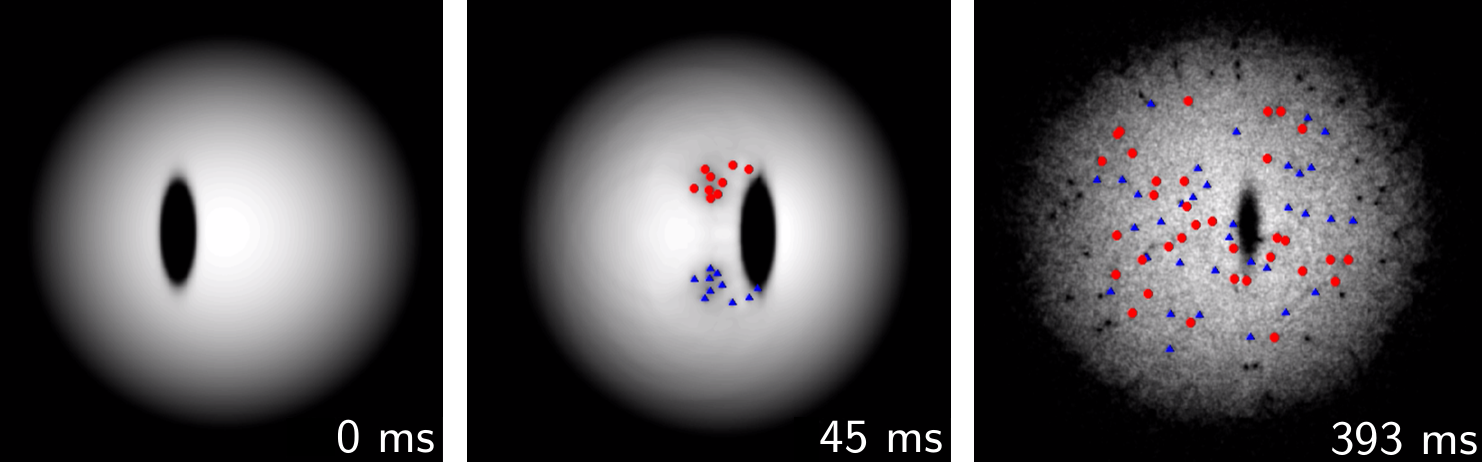
\includegraphics[width=0.9\linewidth]{shin/fig6.png}
\caption{\label{fig:ellipse} Snapshots of the condensate density for a translational of speed $v=0.8$mm/s past an elliptical obstacle (ellipticity $\epsilon=3$). The field of view in each subfigure is of size $[170\mu$m$]^2$ and shifted along the $x$-axis so as to best display the condensate.  Compared to the corresponding snapshots in Figure \ref{fig:densSnapshots}, the elliptical obstacle generates as many final vortices but at a lower translational speed and with reduced condensate disruption.
}
\end{figure}
\section{Conclusions}
In conclusion, we have shown that the recent experimental creation and decay of vortices within a BEC~\citep{kwon_moon_14} is well described by simulations of the 2D GPE with phenomenological dissipation (despite the 3D nature of the system).  Theoretical access to the condensate phase, and thus the circulation of the vortices, promotes our understanding of the dynamics.  In the early stages of 
translation of the obstacle, a quasi-classical wake of vortices 
forms behind it, before symmetry breaking causes disorganisation 
of the vortices.  After the obstacle is removed, 
the vortices decay in a manner which is consistent with the two mechanisms proposed by 
Kwon \etalcc, i.e. loss of vortices at the condensate edge due to thermal dissipation and vortex-antivortex 
annihilation events within the condensate.

We fit the vortex decay the rate equations proposed by Kwon \etal and Cidrim \etal In the case of Kwon's equation we enforce the meaning of the decay rates to find values comparable to the coldest experiments of Kwon \etal In the case of fitting to Cidrim's modified equation, we find rates comparable to the simulations of Cidrim \etal without the need to enforce meaning. We conclude that Cidrim's equation fits to the data most favourably, while providing physically realistic values for the decay rates.

We confirm the occasional appearance of crescent-shaped density features, resulting either from the proximity 
of vortex cores or from a sound pulse which follows a vortex-antivortex reconnection.  Finally, we propose that a moving {\it elliptical} obstacle may provide a cleaner and more efficient means to generate two-dimensional quantum turbulence.

\end{chapter}